
\documentclass[11pt]{article}
% \usepackage[margin=1in]{geometry}
\usepackage{enumerate}
\usepackage{forest}
\usepackage[margin=1in]{geometry}
\usepackage{mathtools}
\usepackage{amsmath}
\usepackage{amssymb}
\usepackage{gensymb}
\usepackage{hyperref}
\usepackage{floatrow}
\floatsetup[table]{capposition=top}

%opening
\title{CSCI 491/591 P2}
\date{March 1, 2016}
\author{Group 4\\Chenglin Fan, Jici Huang,
Angelica Davis, Peng Zou}

\begin{document}

\maketitle
\noindent
We selected an interesting data set among several data sets
that we would like to explore in the project. The data set is one of the GPS trajectories. We will provide the information where the data set is from and explain the meanings of data. We will also conjecture what we might find in this project based on the exploration of the data set.
\section*{Data Set We Chose}
The data set being explored is the GPS trajectories of the city, Berlin. \\
%In P1, we went through all data sets provided by Map Construction Portal and we decided to investigate trajectory data of the tracks in Berlin, large. 
It is a suitable representative data set because the size of the trajectory data is about midway between Chicago and Athens. The size of data set is a reasonably comparable characteristic since the data sets represent overlapping trajectories as well as noisy trajectories. Thus, a mid-sized data set may well represent the noise ratio (either due to noisy trajectories or lack of sampling uniformity).
% Data set choice (8 points). You must select an interesting data set
% that you will investigate in this project. The data set can be real (GPS trajectories,
% Four-square check-ins, gene expressions, March madness brackets,
% baseball statistics, 3D objects, movie scripts, etc.), or it can be theoretical
% (flip graphs, the space of image patches, etc.). [Deliverable: one-to-two page write-up].

\section*{Details About the Data}
The GPS trajectories of Berlin was downloaded from the Map Construction Portal(\url{http://www.mapconstruction.org/data_downloads/}).  \\
The GPS trajectories of Berlin contain the trajectory data of trips in Berlin. Here the trip is a collection of GPS trajectories for one trip over some time period. The trajectory data has more than 27,000 trips in .txt format. \\
Each trip file consists trajectory data of x-coordinate, y-coordinate and time stamp. Table \ref{table:questions} provides a sample of a trip file partially of the trajectory data of Berlin.
% Explain where the data is
% from, what the data means,
% TODO: write something here.\\
% \begin{center}
%  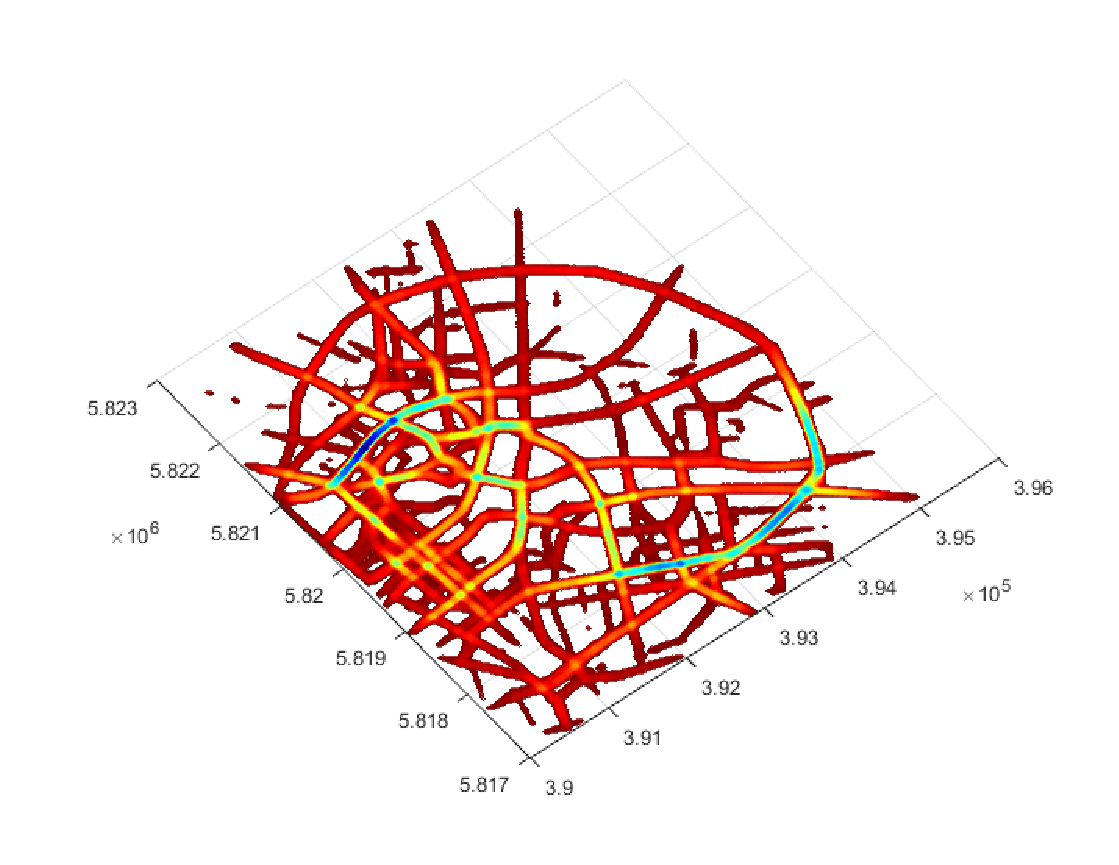
\includegraphics[scale=0.9]{p1.eps} 
% \end{center}
\begin{table}
\begin{center}
\begin{tabular}{ |c |c| c| }
\hline
  x & y & Time stamp   \\ \hline
  393742.586772 & 5821049.184616 & 2585542.00   \\ \hline
  393747.949682 & 5821296.284551 & 2585604.00 \\  \hline
  393883.091662 & 5821448.203015 & 2585677.00  \\ \hline
  393759.343945 & 5821821.259046 & 2585738.00\\ \hline
  \vdots & \vdots & \vdots \\ \hline
\end{tabular}
\end{center}
\caption{An excerpt of trajectory data of Berlin in a trip file}
\label{table:questions}
\end{table}

%\begin{figure}[h!]
 % \caption{A tracking map after processing the track Berlin large data set}
 % \centering
% 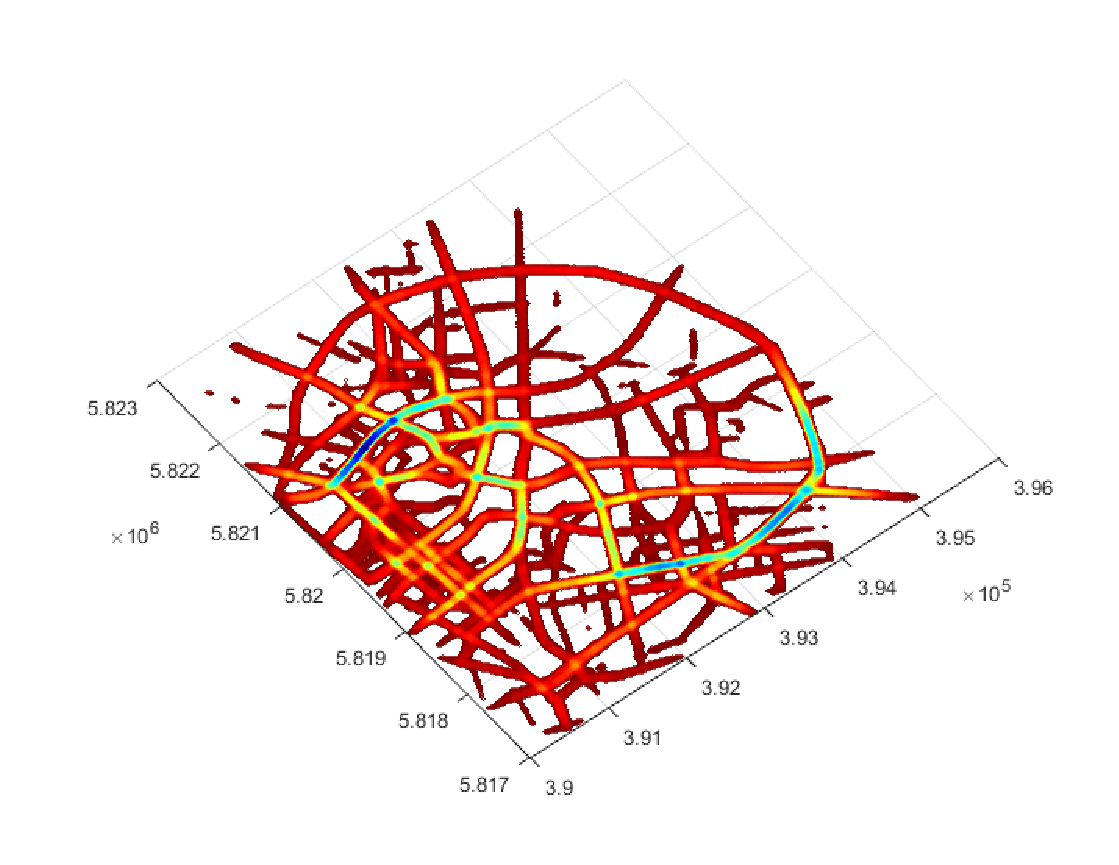
\includegraphics[scale=0.8]{p1.eps} 
%\end{figure}

\pagebreak
\section*{What We Might Find}
We might find out that the trajectory data we chose does not produce any map without using the techniques we mentioned in the previous deliverable. We might come up with a road map of Berlin based on the trajectory data we chose after using the techniques. We might find some new technique by exploring the GPS trajectories data. 
\begin{itemize}
  \item Estimate the underlying road network  by using the trajectory data, as the trajectory data record the track of taxis, which usually run on the road network of the city.
  
  \item  Find the roads with heavy traffic, namely the roads with high density of trajectory.   We also want to analyze the topological structure of the heavy roads in the city.

\end{itemize}





% \section*{Discussion}
% In P2, we had discussion on the analysis of the data. We came up with two data files from the original trip files. \\
% It is usually nice to conclude any write-up.\\

% pts.txt: grid points after the city, 
% manifold value: clr.txt
\section*{Conclusion}
Our group believes that the project is interesting. We are motivated to explore the GPS data by the applications of GPS that are affecting every aspect of modern life. We want to use the topology knowledge in this class to do some thing with application in real life.
% \\
% 1. Using a. b. c. ... as section numbers is not really standard, and looks a little funny to me.  Perhaps just stick with the standard Section Name (maybe you were using an enumeration instead)?{\bfseries FIXED}\\ 
% Use capital letters to start a sentence (e.g., "the description of map data ..."){\bfseries FIXED}\\
% This deliverable was expected to be a bit more narrative in nature.  As it is written, it is closer to an outline than a write-up.\\
% For vertex data: what are the coordinates?  lat/lon or x/y (if lat/lon, you will need to use a local projection to the plane ...)\\
% 'track data' $\rightarrow$ 'trajectory data'\\
%  Captions for tables should always go above the table (for figures, it always goes below the figure).  See this reference: The Elements of Typographic Style){\bfseries FIXED}\\
% While HZ02 is one of the first references on persistence, also take a look at the survey paper: https://users.cs.duke.edu/~edels/Papers/2008-B-02-PersistentHomology.pdf\\
% c.1 and d.1: Persistent is an adjective, so either write "persistent homology" or "persistence" \\
% discrete Morse theory differs from Morse theory in that we no longer require differentiable functions.\\
% Perhaps a description of what is done in [SL15] would be in order.
% Your biblio entries are a little off.  Please check your .bib file (if you don't see why ... send me your .bib file and I can take a look for you).\\
% Are you assuming a manifold somewhere?  I ask because you talk about manifolds ...{\bfseries NA}\\
% Be sure to have your group number in your project deliverables.{\bfseries FIXED}\\
\end{document}
